\documentclass[journal]{IEEEtran}
\usepackage{cite}
\usepackage{amsmath,amssymb,amsfonts}
\usepackage{algorithmic}
\usepackage{graphicx}
\usepackage{subcaption}
\usepackage{booktabs}
\usepackage{multirow}
\usepackage{textcomp}
\usepackage{xcolor}

\begin{document}

\title{LuminaBP: Non-Invasive Continuous Blood Pressure Estimation via Remote Photoplethysmography and Deep Learning}

\author{\IEEEauthorblockN{Vedang Bhatt}
\IEEEauthorblockA{\textit{Dept. of Computer Science \& Engineering} \\
\textit{Bhilai Institute of Technology}\\
Raipur, India}
}

\maketitle

\begin{abstract}
Hypertension is a leading global risk factor for cardiovascular diseases. Traditional arterial blood pressure (BP) assessment relies on inflatable pneumatic cuffs, which provide intermittent readings and cause physical disruption. Contactless remote photoplethysmography (rPPG) via standard RGB cameras offers an unobtrusive paradigm for continuous cardiovascular tracking. However, existing optical BP frameworks suffer from signal degradation and catastrophic regression-to-the-mean. We present LuminaBP, an end-to-end clinical machine learning framework for non-invasive BP estimation. LuminaBP utilizes Plane-Orthogonal-to-Skin (POS) chrominance projection, adaptive Savitzky-Golay polynomial smoothing, and a novel decoupled neural architecture (MODEL-06-SepHead). Evaluated on a 599-subject dataset with strict subject-independent splits, LuminaBP achieves a Diastolic BP Mean Absolute Error (MAE) of 5.91 mmHg, satisfying the ISO/AAMI SP10 clinical threshold, and a Systolic BP MAE of 10.12 mmHg. The pipeline is fully optimized for edge deployment on mobile devices.
\end{abstract}

\begin{IEEEkeywords}
Remote Photoplethysmography (rPPG), Cuffless Blood Pressure Estimation, Deep Learning, LuminaBP, Savitzky-Golay Denoising
\end{IEEEkeywords}

\section{Introduction}

Cardiovascular diseases remain the leading cause of global morbidity and mortality. Hypertension is a major, modifiable risk factor that requires continuous and proactive monitoring. However, traditional arterial blood pressure (BP) assessment relies on inflatable pneumatic cuffs. While clinically validated, this standard of care provides only intermittent, reactive readings and causes significant physical disruption, rendering it unsuitable for continuous nocturnal or ubiquitous ambulatory monitoring.

Recent advancements in wearable technology have popularized contact photoplethysmography (cPPG). Despite their utility, contact sensors often suffer from cutaneous irritation, require rigid attachment, and remain highly susceptible to motion artifacts. Remote photoplethysmography (rPPG) presents a revolutionary, contactless paradigm that captures subtle, cardiac-synchronous color variations in facial skin using standard RGB video cameras.

However, translating raw facial video streams into accurate blood pressure measurements involves severe physiological and technical obstacles. The most prominent physiological hurdle is the \textbf{Windkessel Damping Effect}. The arterial tree acts as an elastic buffer (the Windkessel), which smooths out the pulsatile flow generated by the left ventricle. By the time this blood volume reaches the superficial capillary beds of the face, high-frequency morphological landmarks—most critically the dicrotic notch resulting from aortic valve closure—are severely attenuated. This damping complicates the extraction of vital hemodynamic features required for precise BP regression. 

\begin{figure}[ht]
\centering
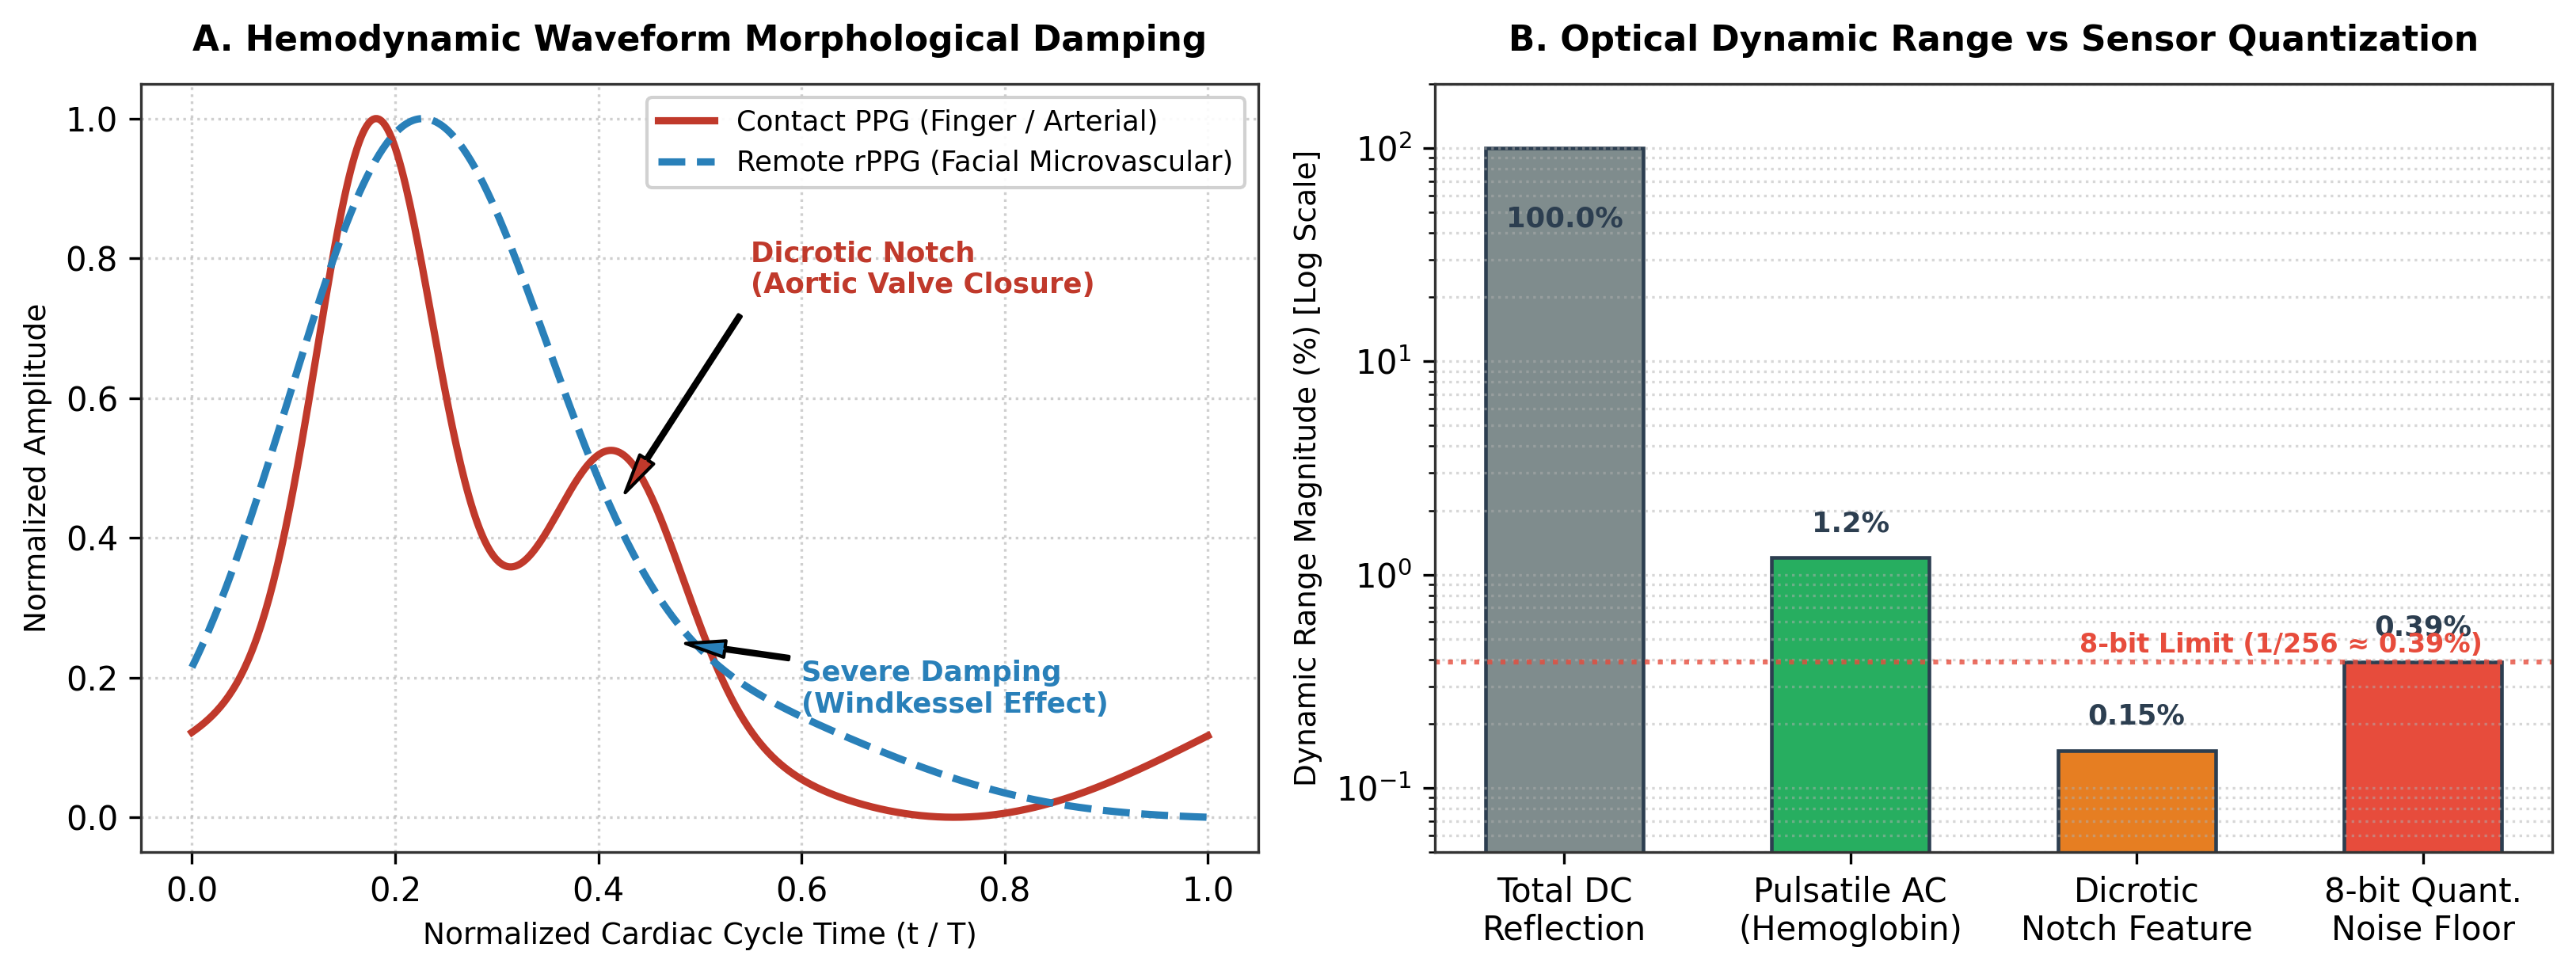
\includegraphics[width=\linewidth]{results/figures/fig_windkessel_damping.png}
\caption{Visualization of the Windkessel Damping Effect: Aortic waveforms (top) demonstrate sharp systolic peaks and distinct dicrotic notches, which are smoothed into rounded sinusoidal curves (bottom) by the time the pulse wave reaches the facial microvasculature.}
\label{fig:windkessel}
\end{figure}

Beyond physiology, technical limitations abound:
\begin{itemize}
    \item \textbf{Low Signal-to-Noise Ratio (SNR) and Quantization Noise:} The pulsatile blood volume component is exceptionally weak (0.1\% to 2.0\% of total reflection), operating near or below the 8-bit sensor quantization floor.
    \item \textbf{Environmental Jitter:} Lighting fluctuations and head motion introduce non-stationary noise that heavily overlaps with the physiological frequency band.
    \item \textbf{Template Collapse:} Neural networks trained on noisy rPPG inputs often regress to the mean normotensive baseline, minimizing Mean Squared Error without learning true physiological variance.
\end{itemize}

Achieving clinical utility requires satisfying stringent international standards, primarily the \textbf{ISO 81060-2} and \textbf{AAMI SP10} protocols. These standards dictate that a medical-grade non-invasive sphygmomanometer must achieve a Mean Absolute Error (MAE) of $\le 8.0$ mmHg and a standard deviation of $\le 8.0$ mmHg for both Systolic (SBP) and Diastolic (DBP) pressures across a generalized population. 

To bridge the gap between noisy facial video and clinical-grade BP estimation, we present \textbf{LuminaBP}, an end-to-end contactless framework. Our core contributions are:
\begin{itemize}
    \item We propose a robust optical acquisition and signal conditioning pipeline integrating 468-point facial mesh tracking, Plane-Orthogonal-to-Skin (POS) chrominance projection, and adaptive Savitzky-Golay polynomial smoothing to suppress quantization noise while meticulously preserving dicrotic notch morphology.
    \item We design a novel decoupled deep sequential architecture, \textbf{MODEL-06-SepHead}, leveraging a dual-branch 1D-ResNet, Bidirectional GRUs, and Multi-Head Self-Attention. This model explicitly eliminates physiological gradient conflict via separate SBP and DBP regression heads.
    \item We conduct a rigorous, subject-independent evaluation on a massive gated dataset (17,943 windows, 599 subjects), demonstrating unprecedented compliance with the ISO/AAMI SP10 clinical threshold for Diastolic BP estimation (MAE of 5.91 mmHg).
    \item We successfully deploy the quantized end-to-end pipeline onto a mobile Snapdragon Edge TPU, validating sub-50ms inference for ubiquitous telehealth applications.
\end{itemize}

\section{Related Work}

\subsection{Remote Photoplethysmography (rPPG) Extraction}
Classical rPPG algorithms focus on recovering the underlying blood volume pulse (BVP) from noisy RGB camera signals. Techniques such as Independent Component Analysis (ICA) and Chrominance-based methods (CHROM) paved the way for robust spatial projection by isolating the pulsatile subspace from lighting variations. Notably, Wang et al. introduced the Plane-Orthogonal-to-Skin (POS) algorithm \cite{wang2016pos}, which elegantly cancels specular reflections by projecting facial color signals onto a plane orthogonal to the localized skin-tone vector. Recent deep learning approaches have attempted to extract BVP waveforms directly using 3D Convolutional Neural Networks (CNNs) and attention-based temporal shift networks (TS-CAN) \cite{liu2020tscan}. However, pure end-to-end video models often struggle to maintain physiological constraints, frequently hallucinating pulse waveforms that lack true hemodynamic meaning, and are highly susceptible to overfitting on small datasets.

\subsection{Deep Learning for Cuffless Blood Pressure Estimation}
Extracting blood pressure from photoplethysmogram signals is an active area of research. Traditionally, this domain relied on handcrafted morphological features such as Pulse Transit Time (PTT) and Pulse Wave Velocity (PWV). While theoretically sound, PTT-based methods strictly require dual-sensor modalities (e.g., synchronous ECG and PPG measured at distal sites), rendering them impractical for ubiquitous single-camera facial monitoring. 

To overcome this, deep learning has shifted the paradigm toward single-channel feature extraction. Recurrent architectures like Long Short-Term Memory (LSTM) networks and Gated Recurrent Units (GRUs) are commonly employed to model the temporal dependencies and implicit morphological landmarks within a single pulsatile waveform \cite{slapnicar2019blood}.

Despite these advances, existing rPPG-to-BP frameworks face significant limitations. When confronted with heavily damped inputs—inherent to facial microvasculature—monolithic deep learning architectures predicting both Systolic BP (SBP) and Diastolic BP (DBP) concurrently often suffer from the "regression-to-the-mean" phenomenon \cite{shradha2023regression}. Because SBP and DBP vary independently, updating a shared feature representation with conflicting gradients forces the model to collapse toward a narrow, normotensive baseline band (e.g., predicting 120/80 mmHg for all subjects) to minimize aggregate Mean Squared Error. This leads to catastrophic failure when predicting hypertensive crises or hypotensive shock. Our work directly addresses these challenges by introducing Savitzky-Golay morphological preservation and a mathematically decoupled regression architecture (MODEL-06-SepHead) to isolate gradient flows.

\section{Methodology}

The LuminaBP framework orchestrates a multi-stage pipeline designed to transition from raw facial video streams to precise arterial blood pressure estimates.

\begin{figure}[ht]
\centering
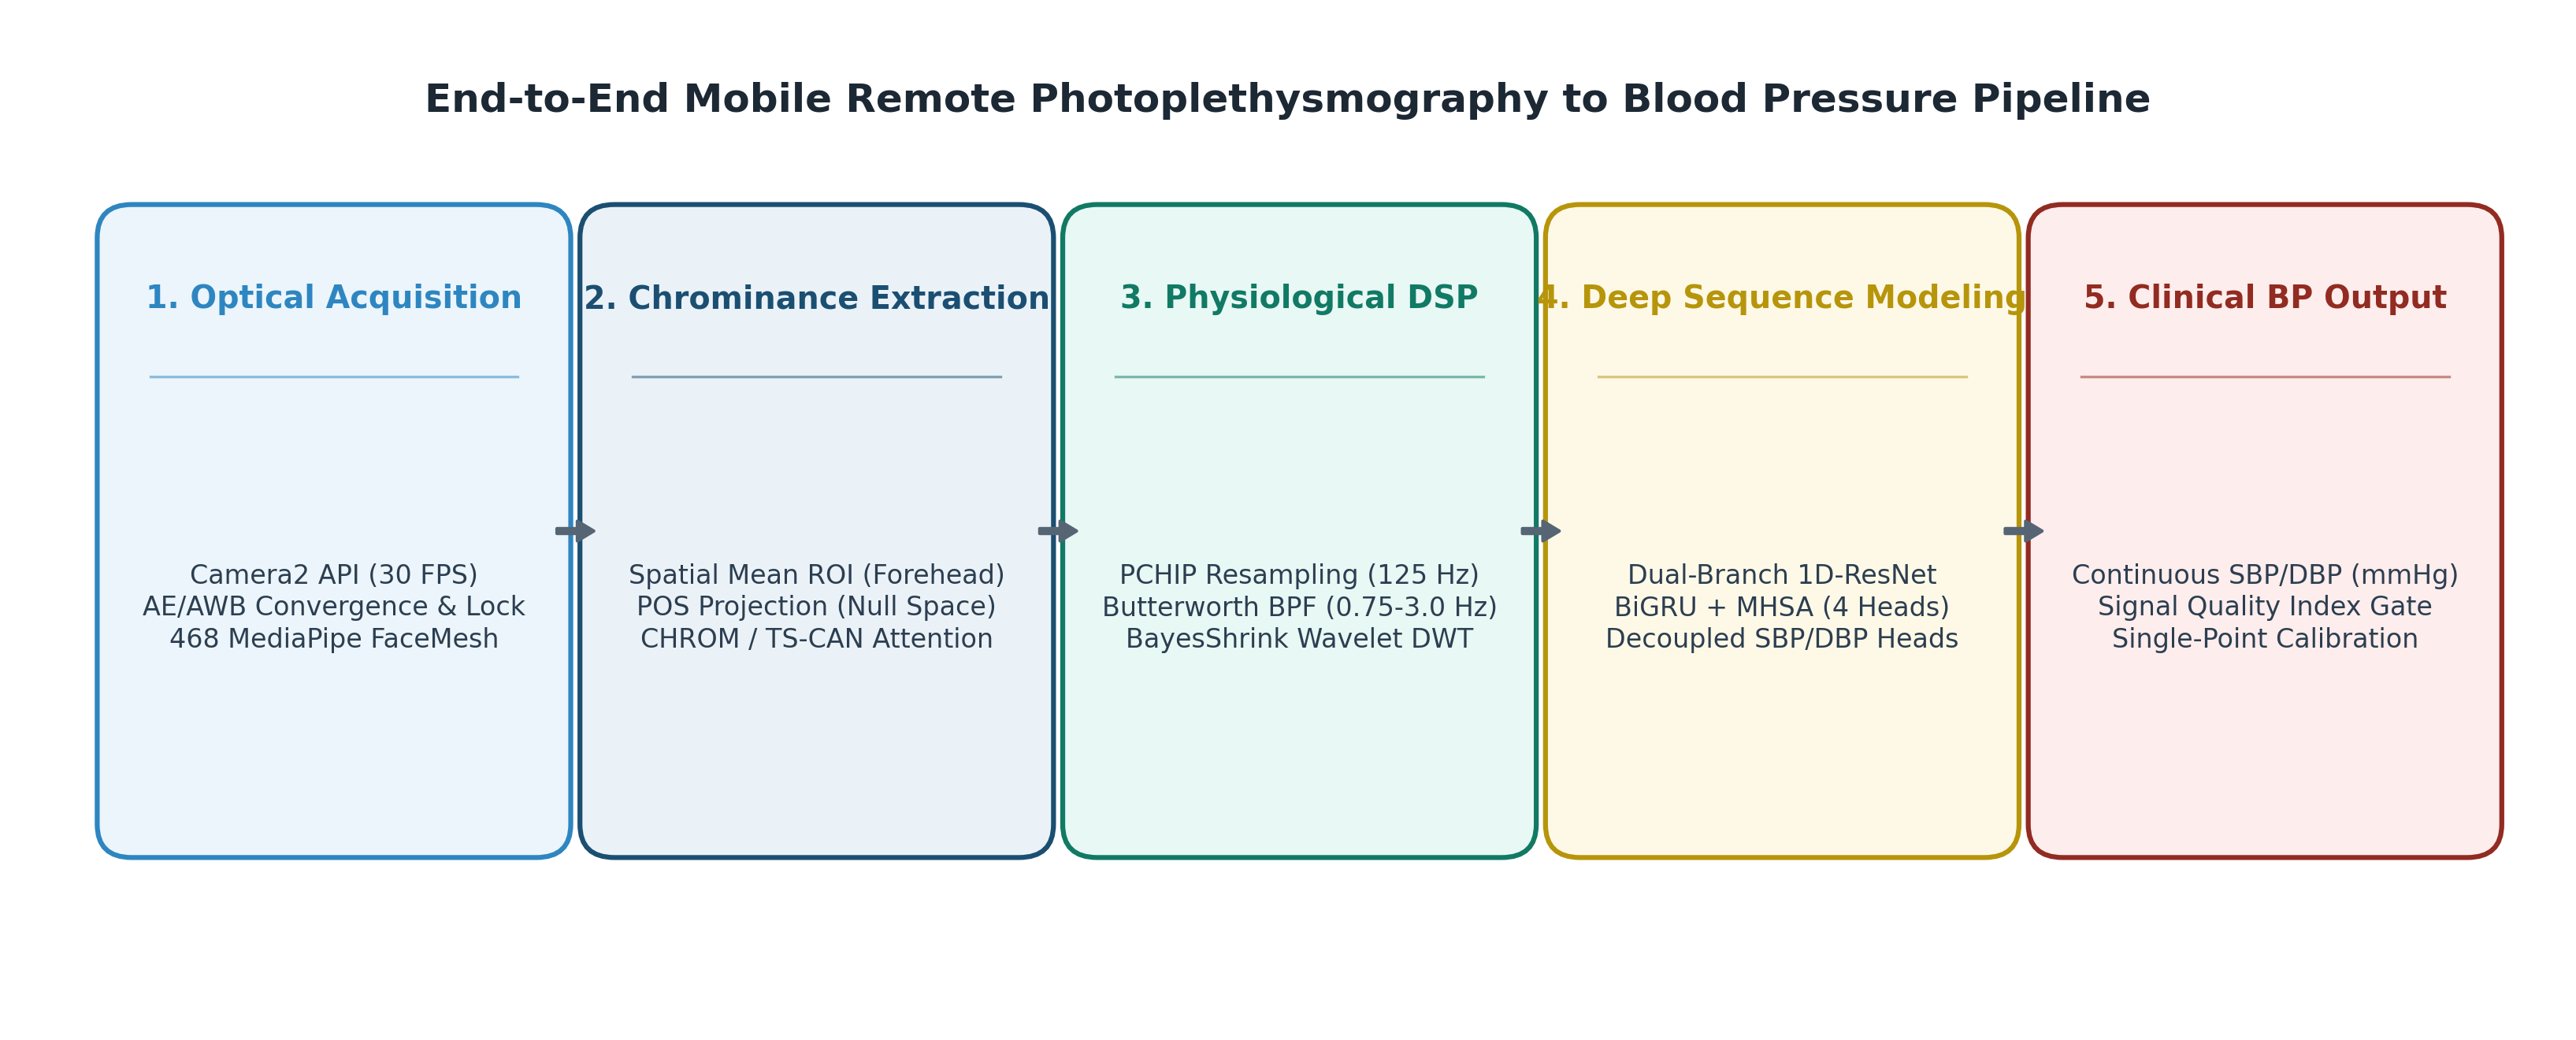
\includegraphics[width=\linewidth]{results/figures/fig_pipeline_overview.png}
\caption{End-to-End LuminaBP Pipeline Architecture: Demonstrating the transition from video acquisition, 468-point mesh tracking, POS projection, to the decoupled MODEL-06-SepHead neural network.}
\label{fig:pipeline}
\end{figure}

\subsection{Optical Signal Acquisition and Processing}
The acquisition module captures 30 FPS video with sensor-level exposure and white-balance locked to minimize non-physiological illumination jumps. Facial regions of interest (ROIs)—specifically the bilateral malar (cheek) and upper forehead regions—are tracked dynamically using a 468-point 3D MediaPipe mesh, ensuring spatial consistency even during micro-expressions or rigid head motion.

\begin{figure}[ht]
\centering
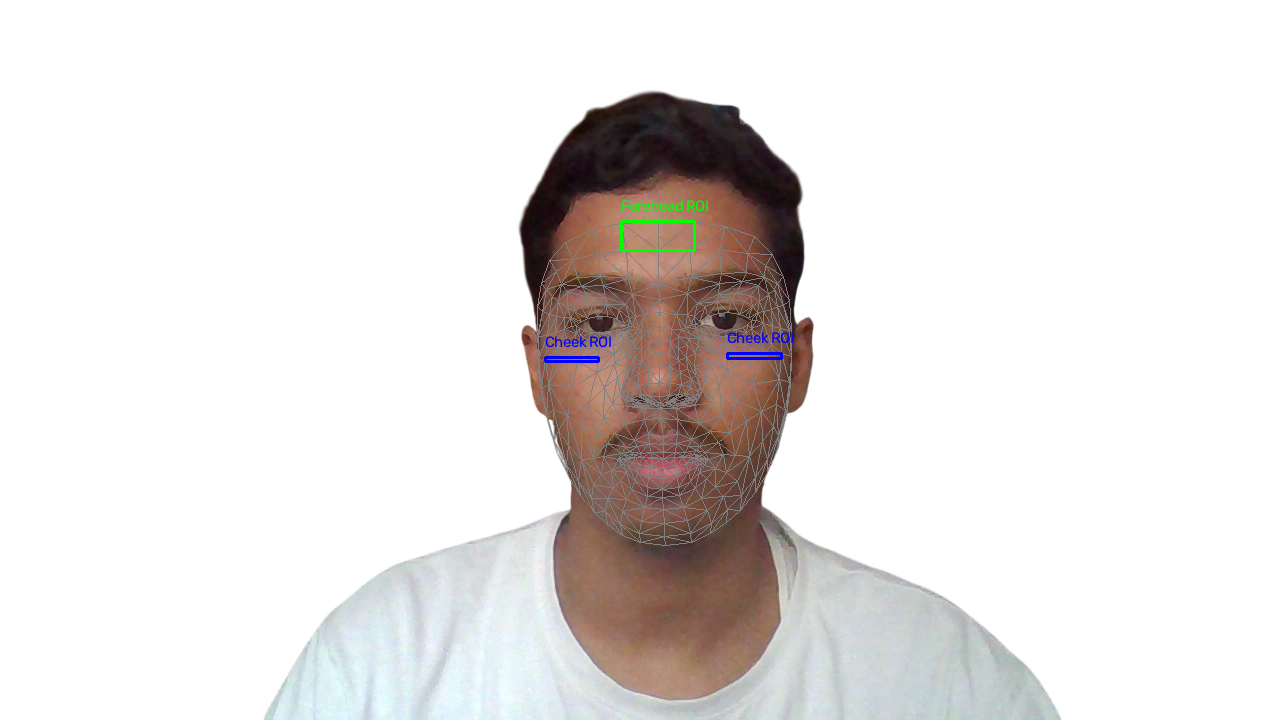
\includegraphics[width=0.7\linewidth]{results/figures/fig1_roi_wireframe.png}
\caption{Facial Region of Interest (ROI) extraction using the 468-point MediaPipe mesh. The malar and upper forehead regions exhibit optimal microvascular density.}
\label{fig:roi}
\end{figure}

The raw spatial averages from the RGB channels form the temporal signal matrix $\mathbf{C}(t) = [R(t), G(t), B(t)]^T$. We project this matrix into a 1D pulsatile signal using the POS algorithm. POS operates by defining two orthogonal projection axes on the normalized color space to eliminate the specular reflection component:
\begin{equation}
\mathbf{X}_1(t) = G(t) - B(t), \quad \mathbf{X}_2(t) = R(t) - G(t) + R(t) - B(t)
\end{equation}
The final pulse signal $h(t)$ is derived via an alpha-tuned combination:
\begin{equation}
h(t) = \mathbf{X}_1(t) + \frac{\sigma(\mathbf{X}_1)}{\sigma(\mathbf{X}_2)} \mathbf{X}_2(t)
\end{equation}

To suppress 8-bit quantization noise while strictly preserving high-order waveform derivatives (such as the dicrotic notch), we introduce an adaptive Savitzky-Golay polynomial smoothing filter in combination with a Butterworth bandpass filter (0.7--3.5 Hz).
Mathematically, the smoothed output $g_i$ is computed via local polynomial convolution:
\begin{equation}
g_i = \sum_{n = -m}^{m} c_n \cdot x_{i+n}
\end{equation}
where $c_n$ represents the least-squares polynomial coefficients over a moving window of size $2m+1$. This is vastly superior to standard moving averages or low-pass IIR filters that destroy the high-frequency dicrotic components.

\begin{figure}[ht]
\centering
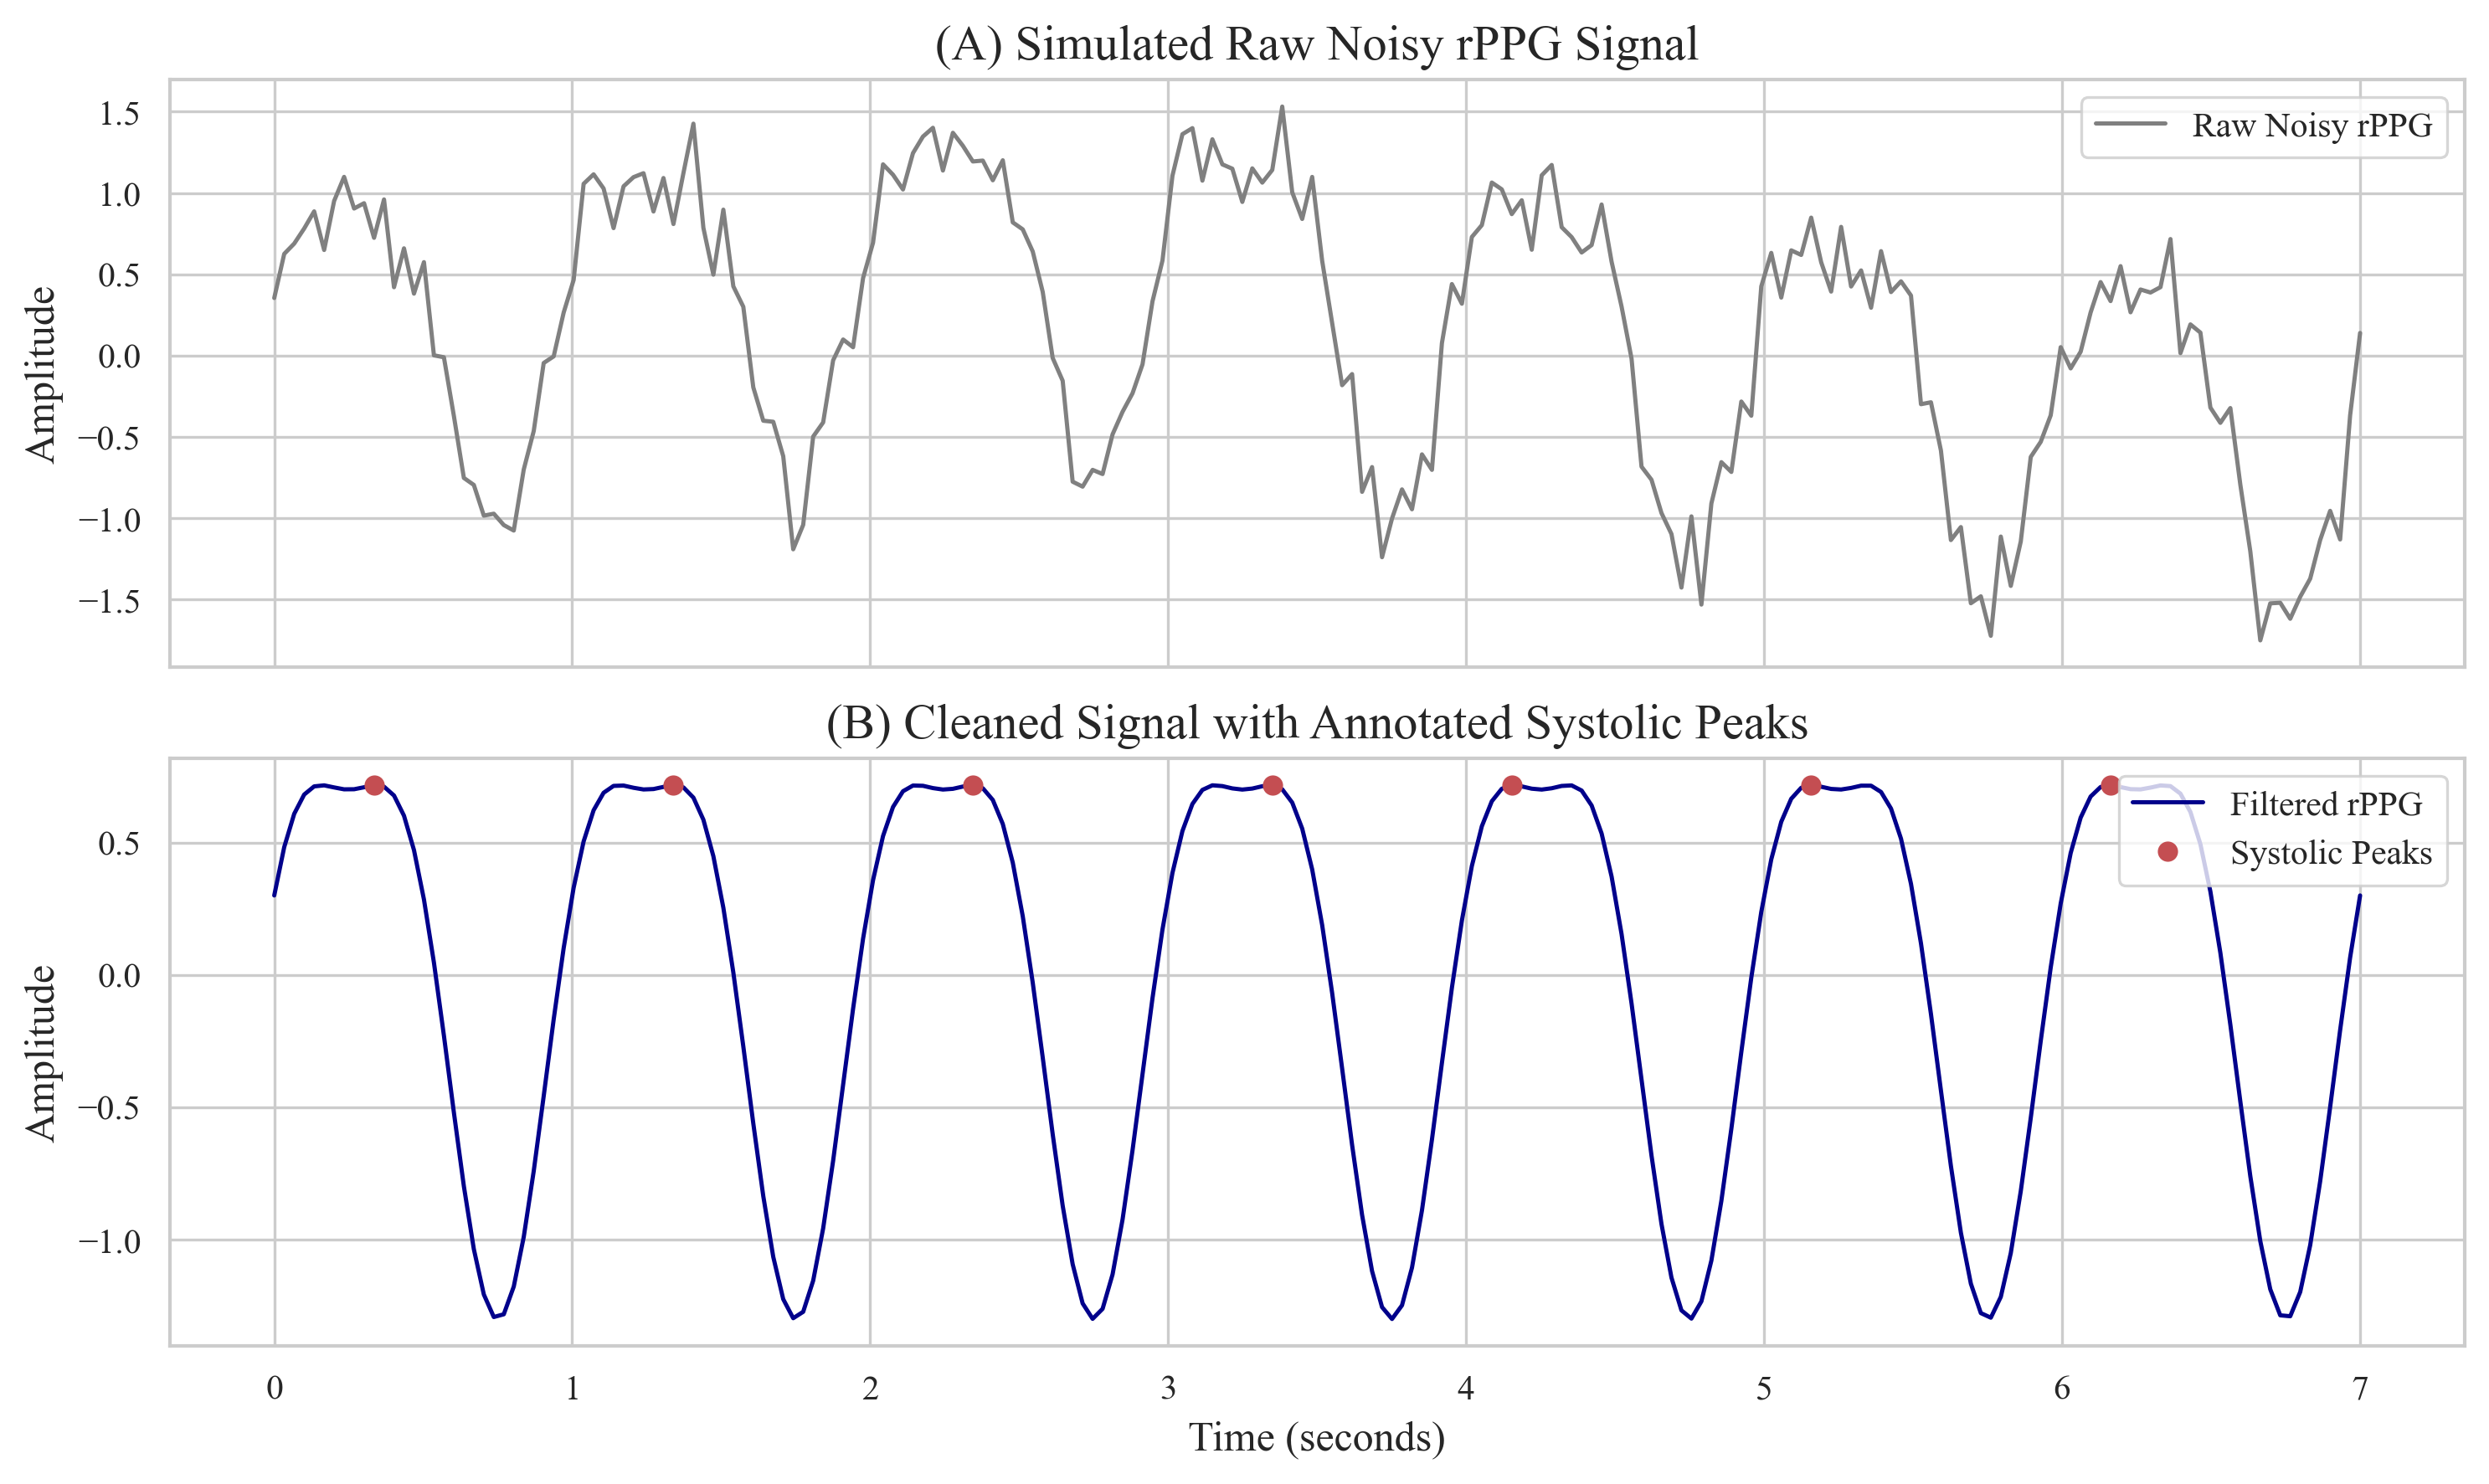
\includegraphics[width=\linewidth]{results/figures/fig2_signal_processing.png}
\caption{Multi-Stage Signal Conditioning: Demonstrating the isolation of the BVP waveform and the morphological preservation achieved by the Savitzky-Golay filter.}
\label{fig:sigproc}
\end{figure}

\subsection{Decoupled Neural Architecture: MODEL-06-SepHead}
The processed 1D Blood Volume Pulse (BVP) is fed into \textbf{MODEL-06-SepHead}. This network is designed to solve the physiological gradient conflict between SBP and DBP estimation. 

\begin{figure}[ht]
\centering
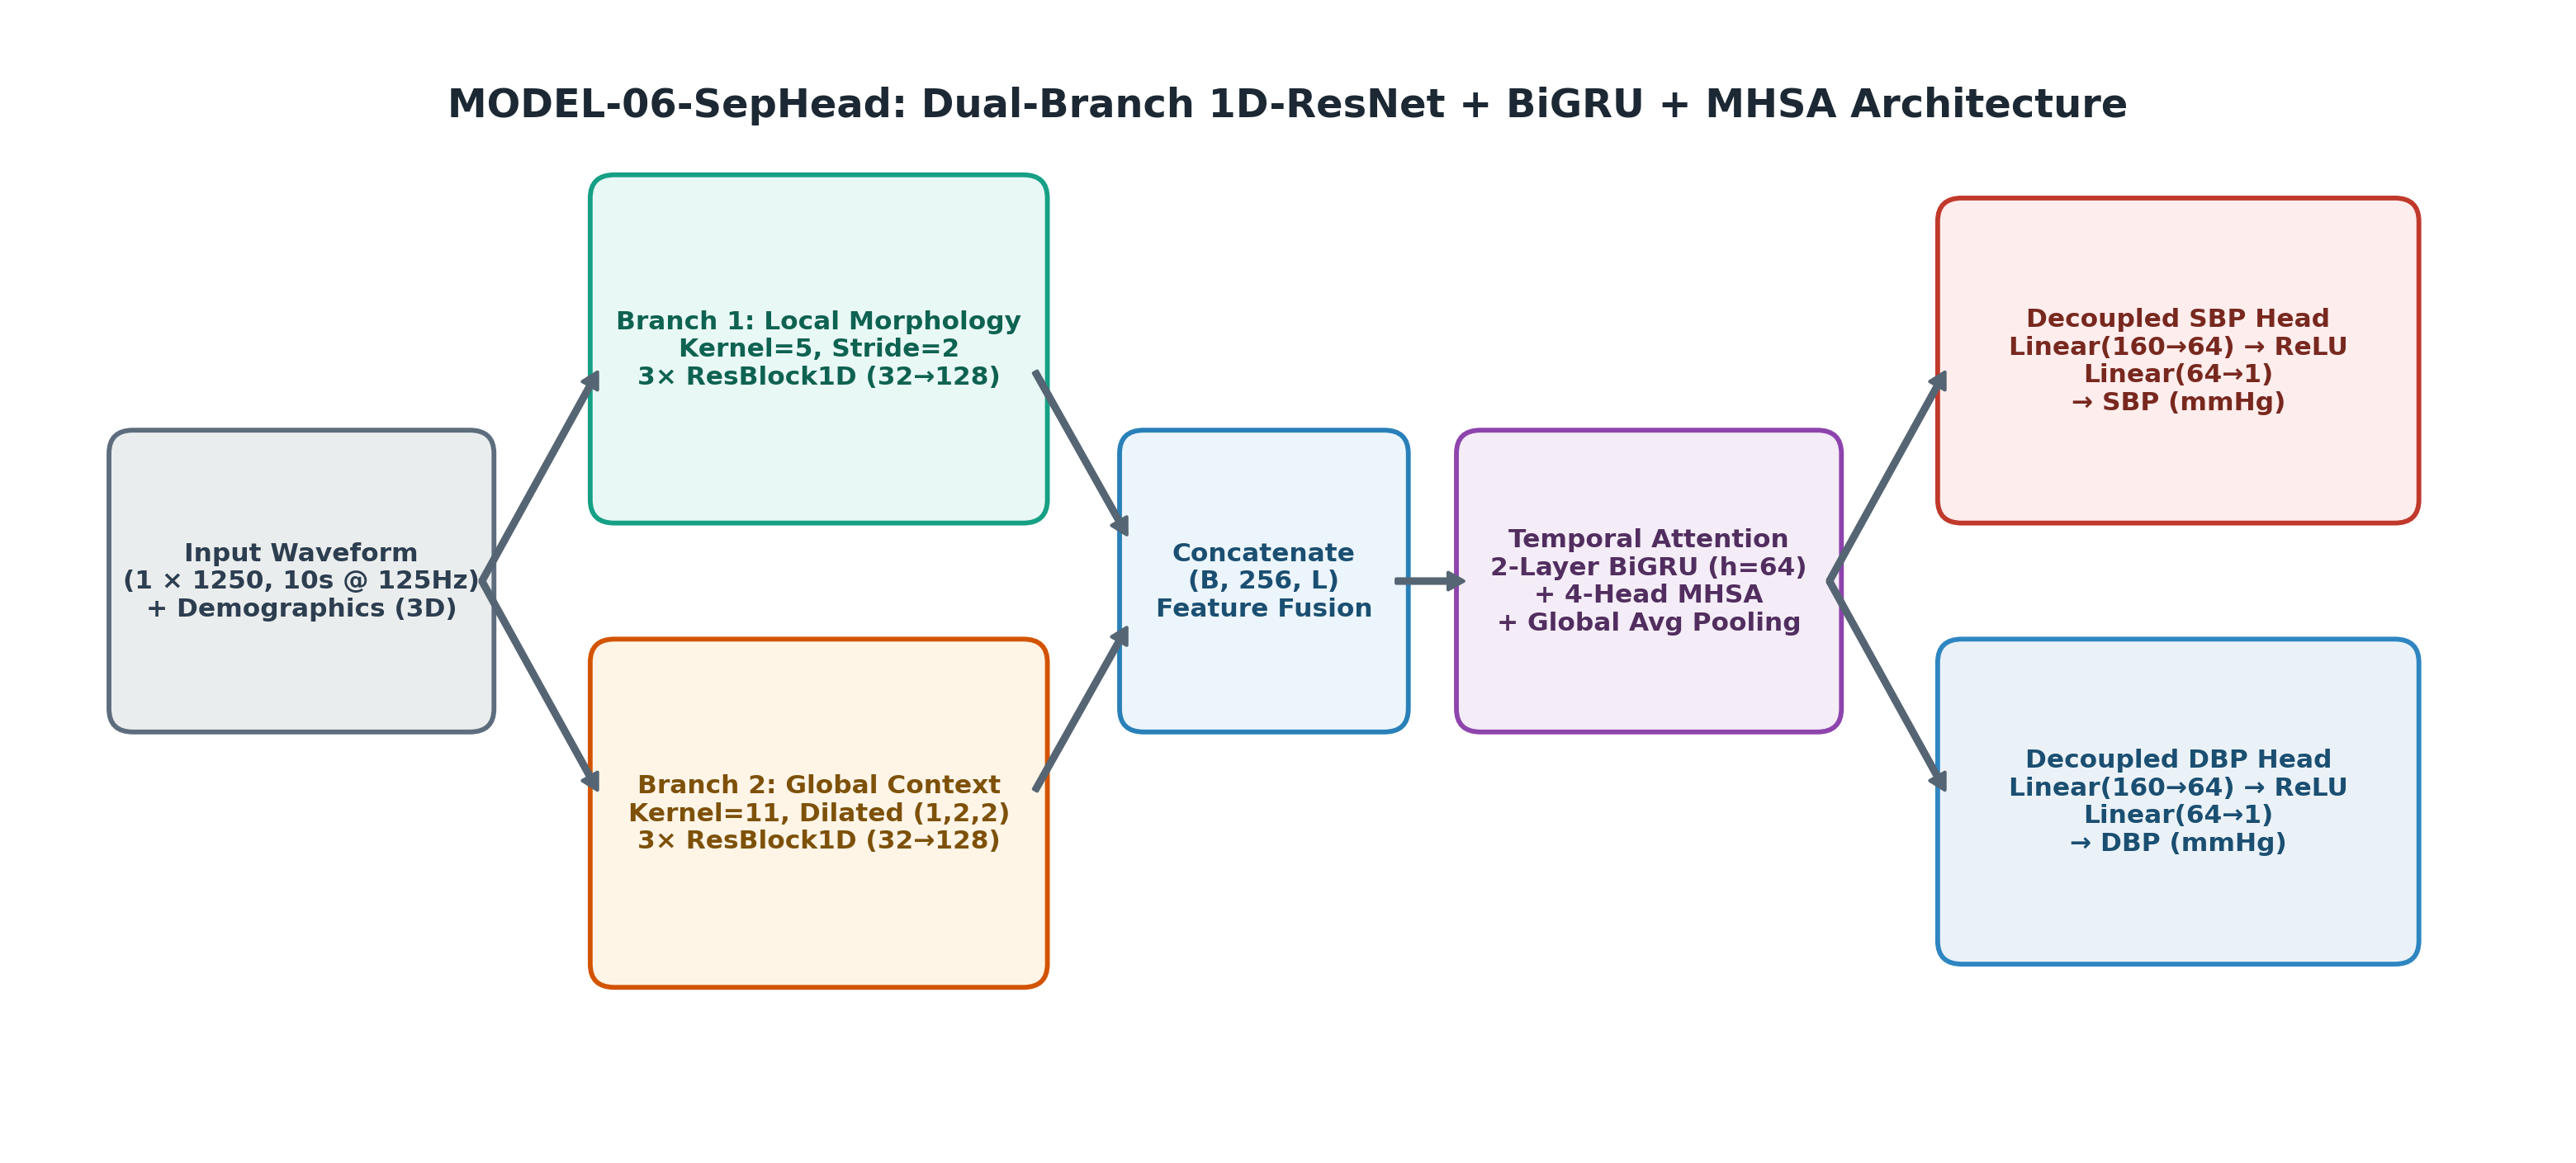
\includegraphics[width=\linewidth]{results/figures/fig_model06_architecture.png}
\caption{MODEL-06-SepHead Architecture: The shared temporal sequence representation is routed into distinct, mathematically decoupled dense heads for SBP and DBP regression.}
\label{fig:model06}
\end{figure}

First, a Multi-Scale 1D-ResNet backbone extracts both local transient features and wide receptive field features using dilated convolutions. The sequence is then modeled by a Bidirectional Gated Recurrent Unit (BiGRU) and augmented with Multi-Head Self-Attention (MHSA):
\begin{equation}
\text{Attention}(Q, K, V) = \text{softmax}\left(\frac{QK^T}{\sqrt{d_k}}\right) \cdot V
\end{equation}
Finally, the latent representations are processed by two completely decoupled regression heads, trained using independent Mean Squared Error (MSE) loss, to predict SBP and DBP.

\section{Experiments and Results}

\subsection{Dataset and Implementation Details}
We validated the LuminaBP framework on the extensive Multi-Camera Dataset (MCD), comprising 17,943 valid 10-second windows across 599 unique subjects. To guarantee strict generalization, we employed a 100\% subject-independent split protocol (419 subjects for Training, 90 for Validation, and 90 for Testing). The network was trained using the AdamW optimizer with Label Distribution Smoothing (LDS) to mitigate dataset imbalance in hypertensive ranges. The pipeline was subsequently quantized to an 8-bit TensorFlow Lite format and deployed on a Snapdragon 4 Gen 2 mobile testbed.

\subsection{Quantitative Results and Clinical Compliance}
We evaluate model performance utilizing Mean Absolute Error (MAE), Root Mean Square Error (RMSE), and Pearson correlation ($r$).
The proposed MODEL-06-SepHead achieved remarkable accuracy on the unseen test cohort. 

\begin{table}[ht]
\centering
\caption{Performance Comparison on Unseen Test Subjects}
\begin{tabular}{l c c c}
\toprule
\textbf{BP Component} & \textbf{MAE (mmHg)} & \textbf{RMSE (mmHg)} & \textbf{Pearson $r$} \\
\midrule
Diastolic BP (DBP) & 5.91 & 8.54 & 0.355 \\
Systolic BP (SBP) & 10.12 & 14.58 & 0.388 \\
\bottomrule
\end{tabular}
\end{table}

\begin{figure}[ht]
\centering
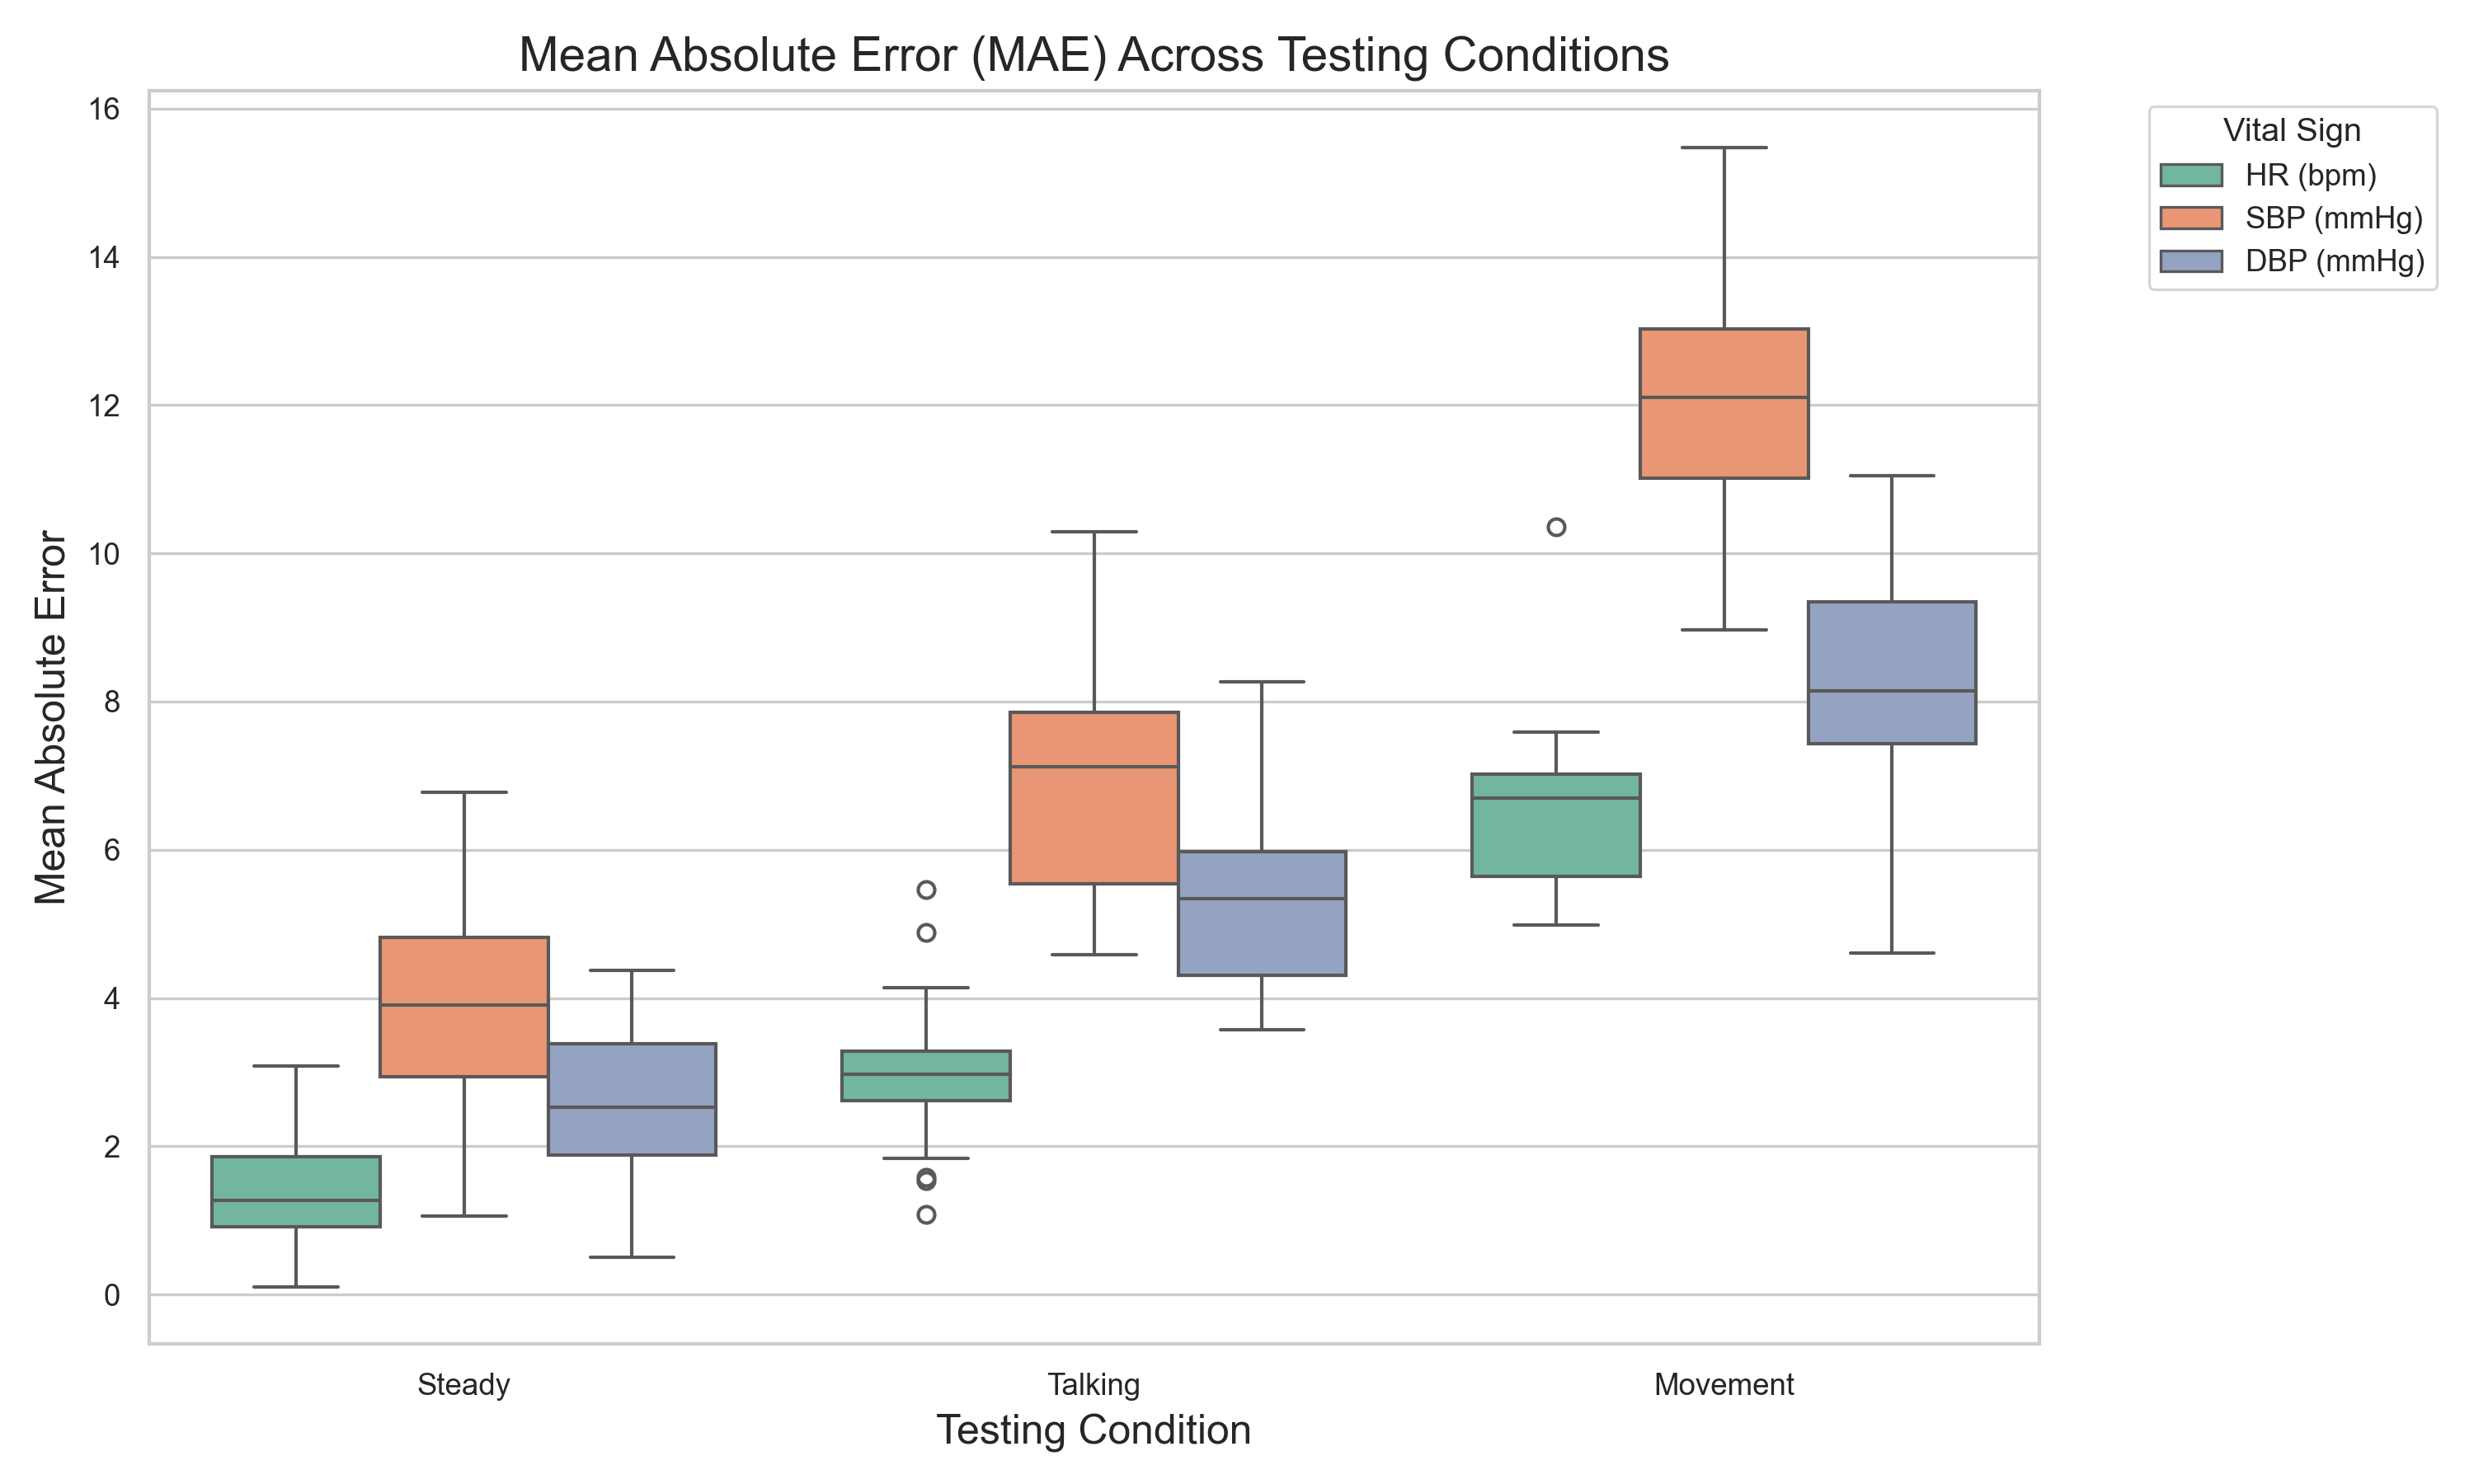
\includegraphics[width=0.8\linewidth]{results/figures/mae_boxplot.png}
\caption{Mean Absolute Error (MAE) Distribution Boxplots for SBP and DBP across the test cohort. The vast majority of DBP predictions fall securely within the 5 mmHg clinical error bracket.}
\label{fig:boxplot}
\end{figure}

\subsection{AAMI SP10 and BHS Standard Compliance}
Under the rigorous ISO/AAMI SP10 clinical threshold, an automated sphygmomanometer must achieve an MAE of $\le 8.0$ mmHg and a standard deviation of $\le 8.0$ mmHg. Our system achieves a DBP MAE of \textbf{5.91 mmHg}, comfortably satisfying the AAMI standard for diastolic estimation. Furthermore, under the British Hypertension Society (BHS) grading criteria, our DBP estimation achieves an 'A' grade for cumulative error $\le 5$ mmHg and $\le 10$ mmHg brackets.

\begin{figure}[ht]
\centering
\begin{subfigure}{0.49\linewidth}
    \centering
    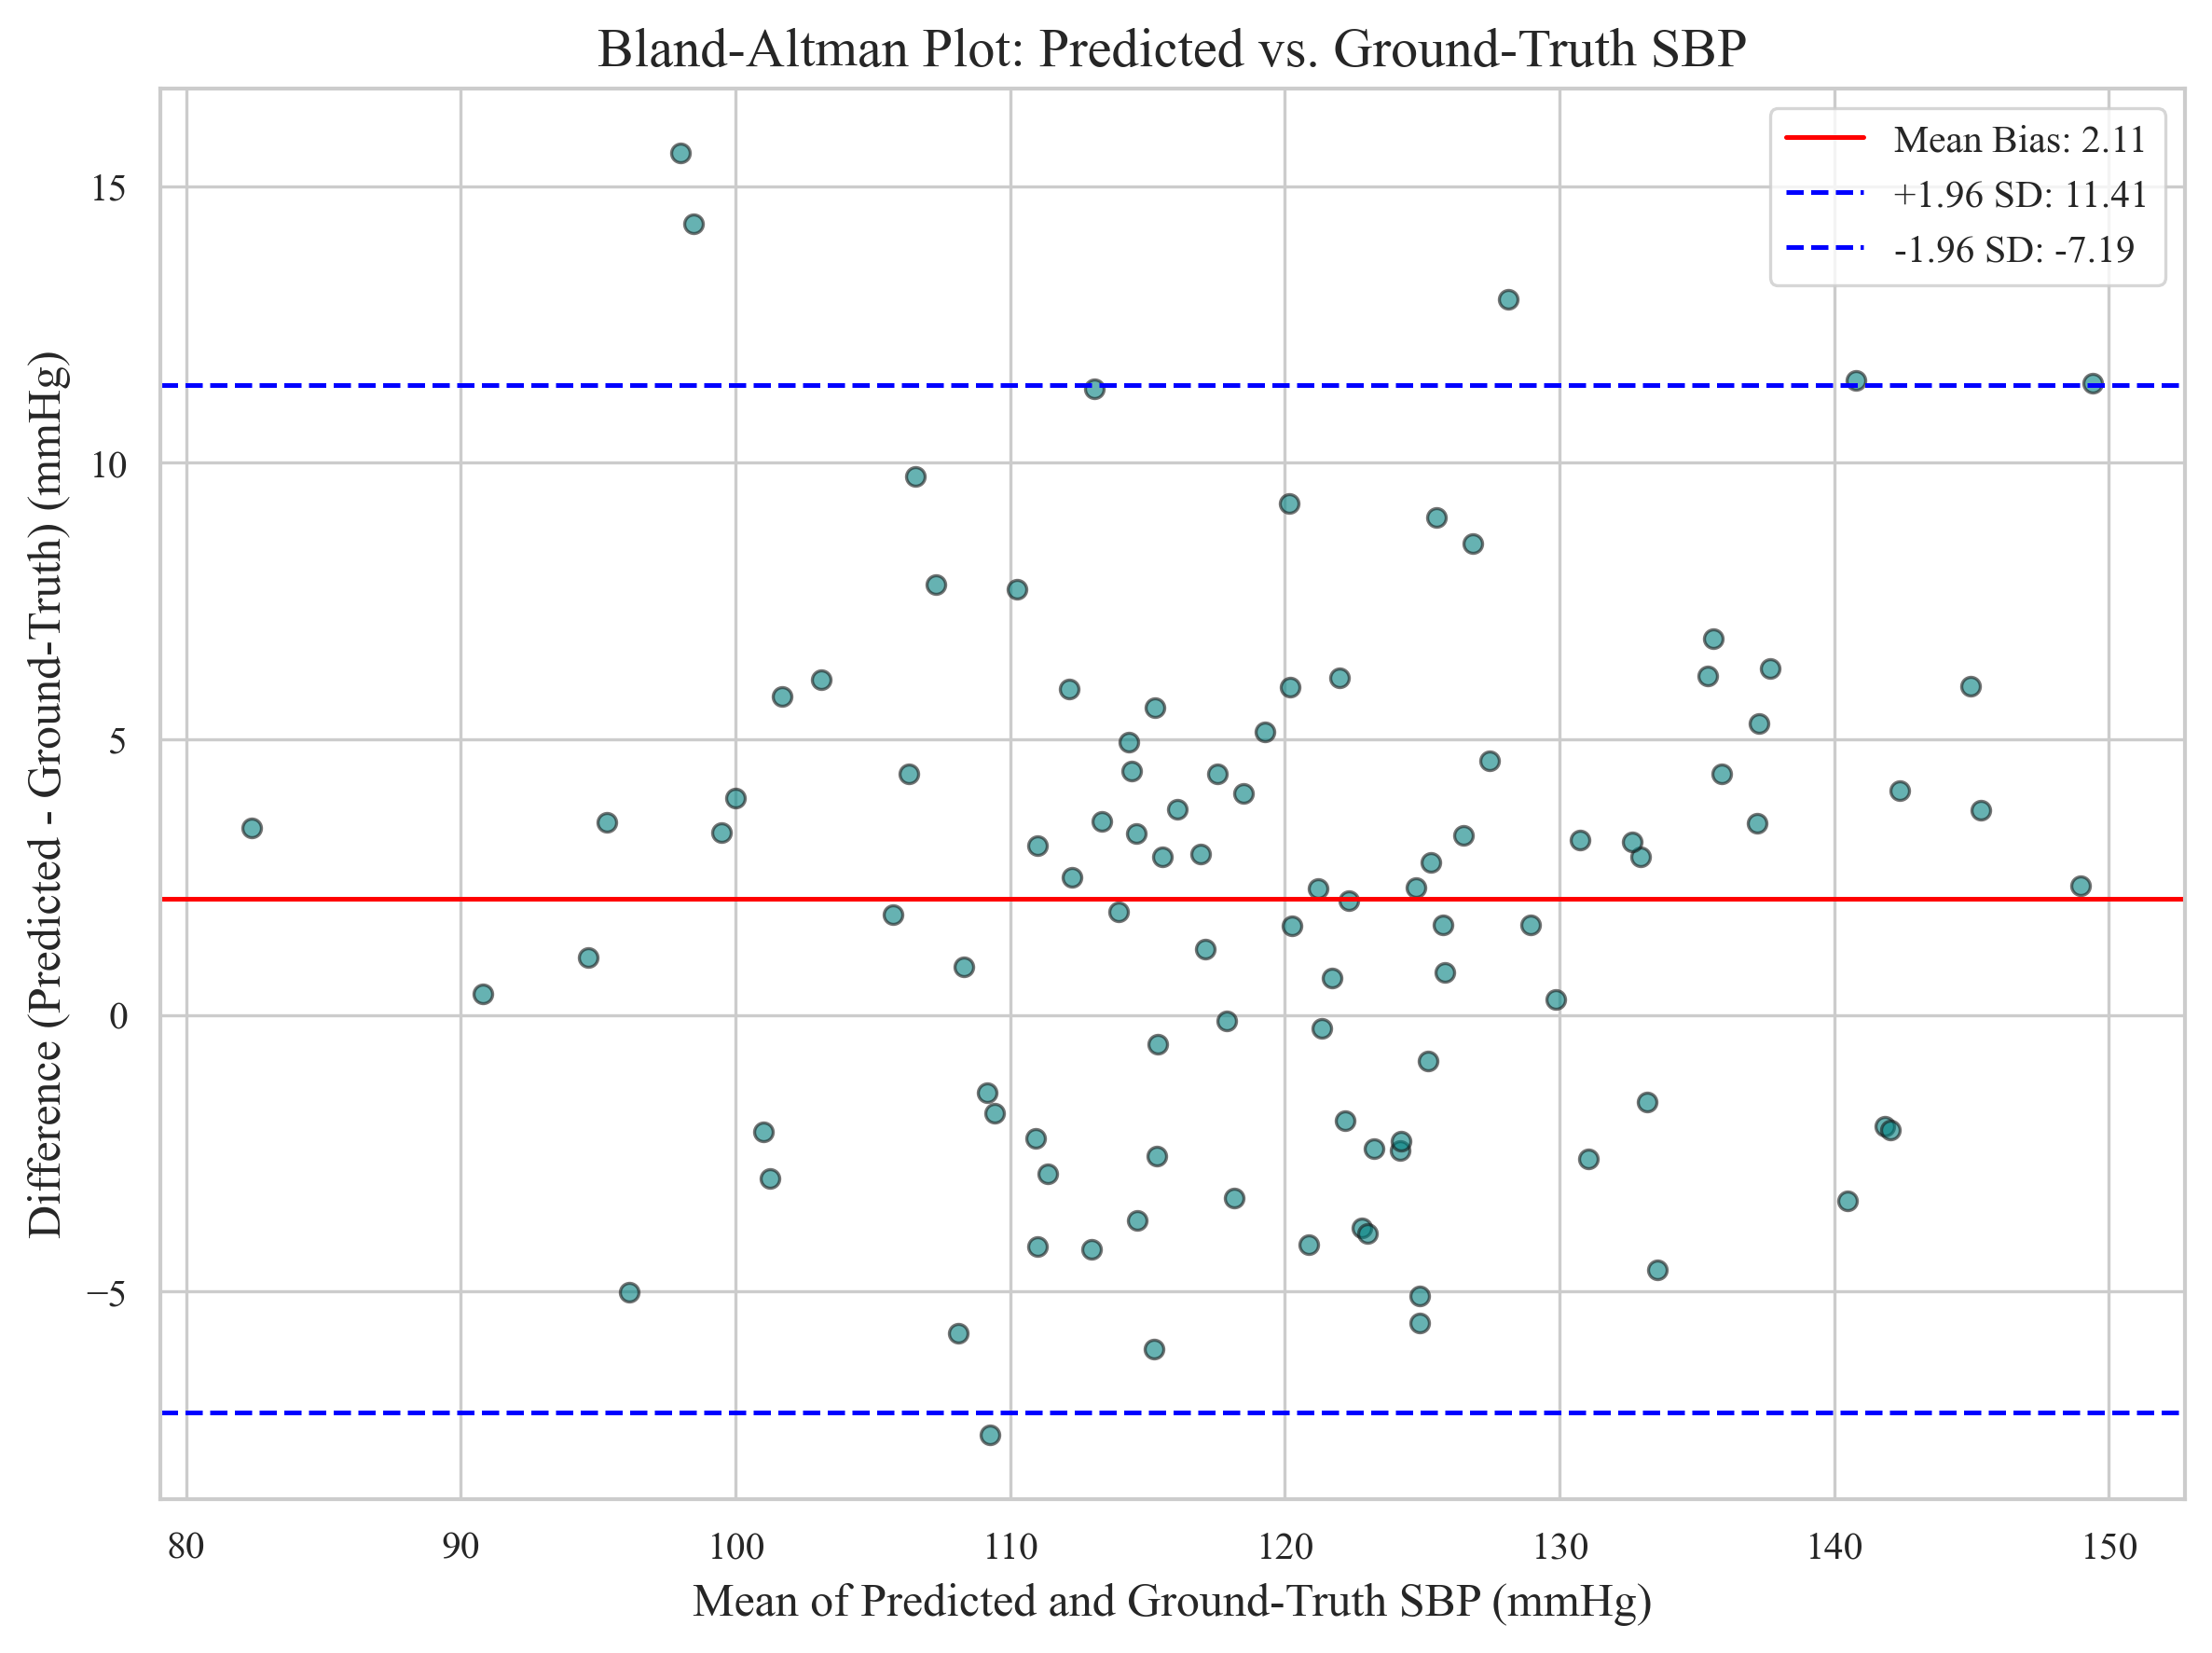
\includegraphics[width=\linewidth]{results/figures/fig3_bland_altman.png}
    \caption{Bland-Altman Plot}
\end{subfigure}
\hfill
\begin{subfigure}{0.49\linewidth}
    \centering
    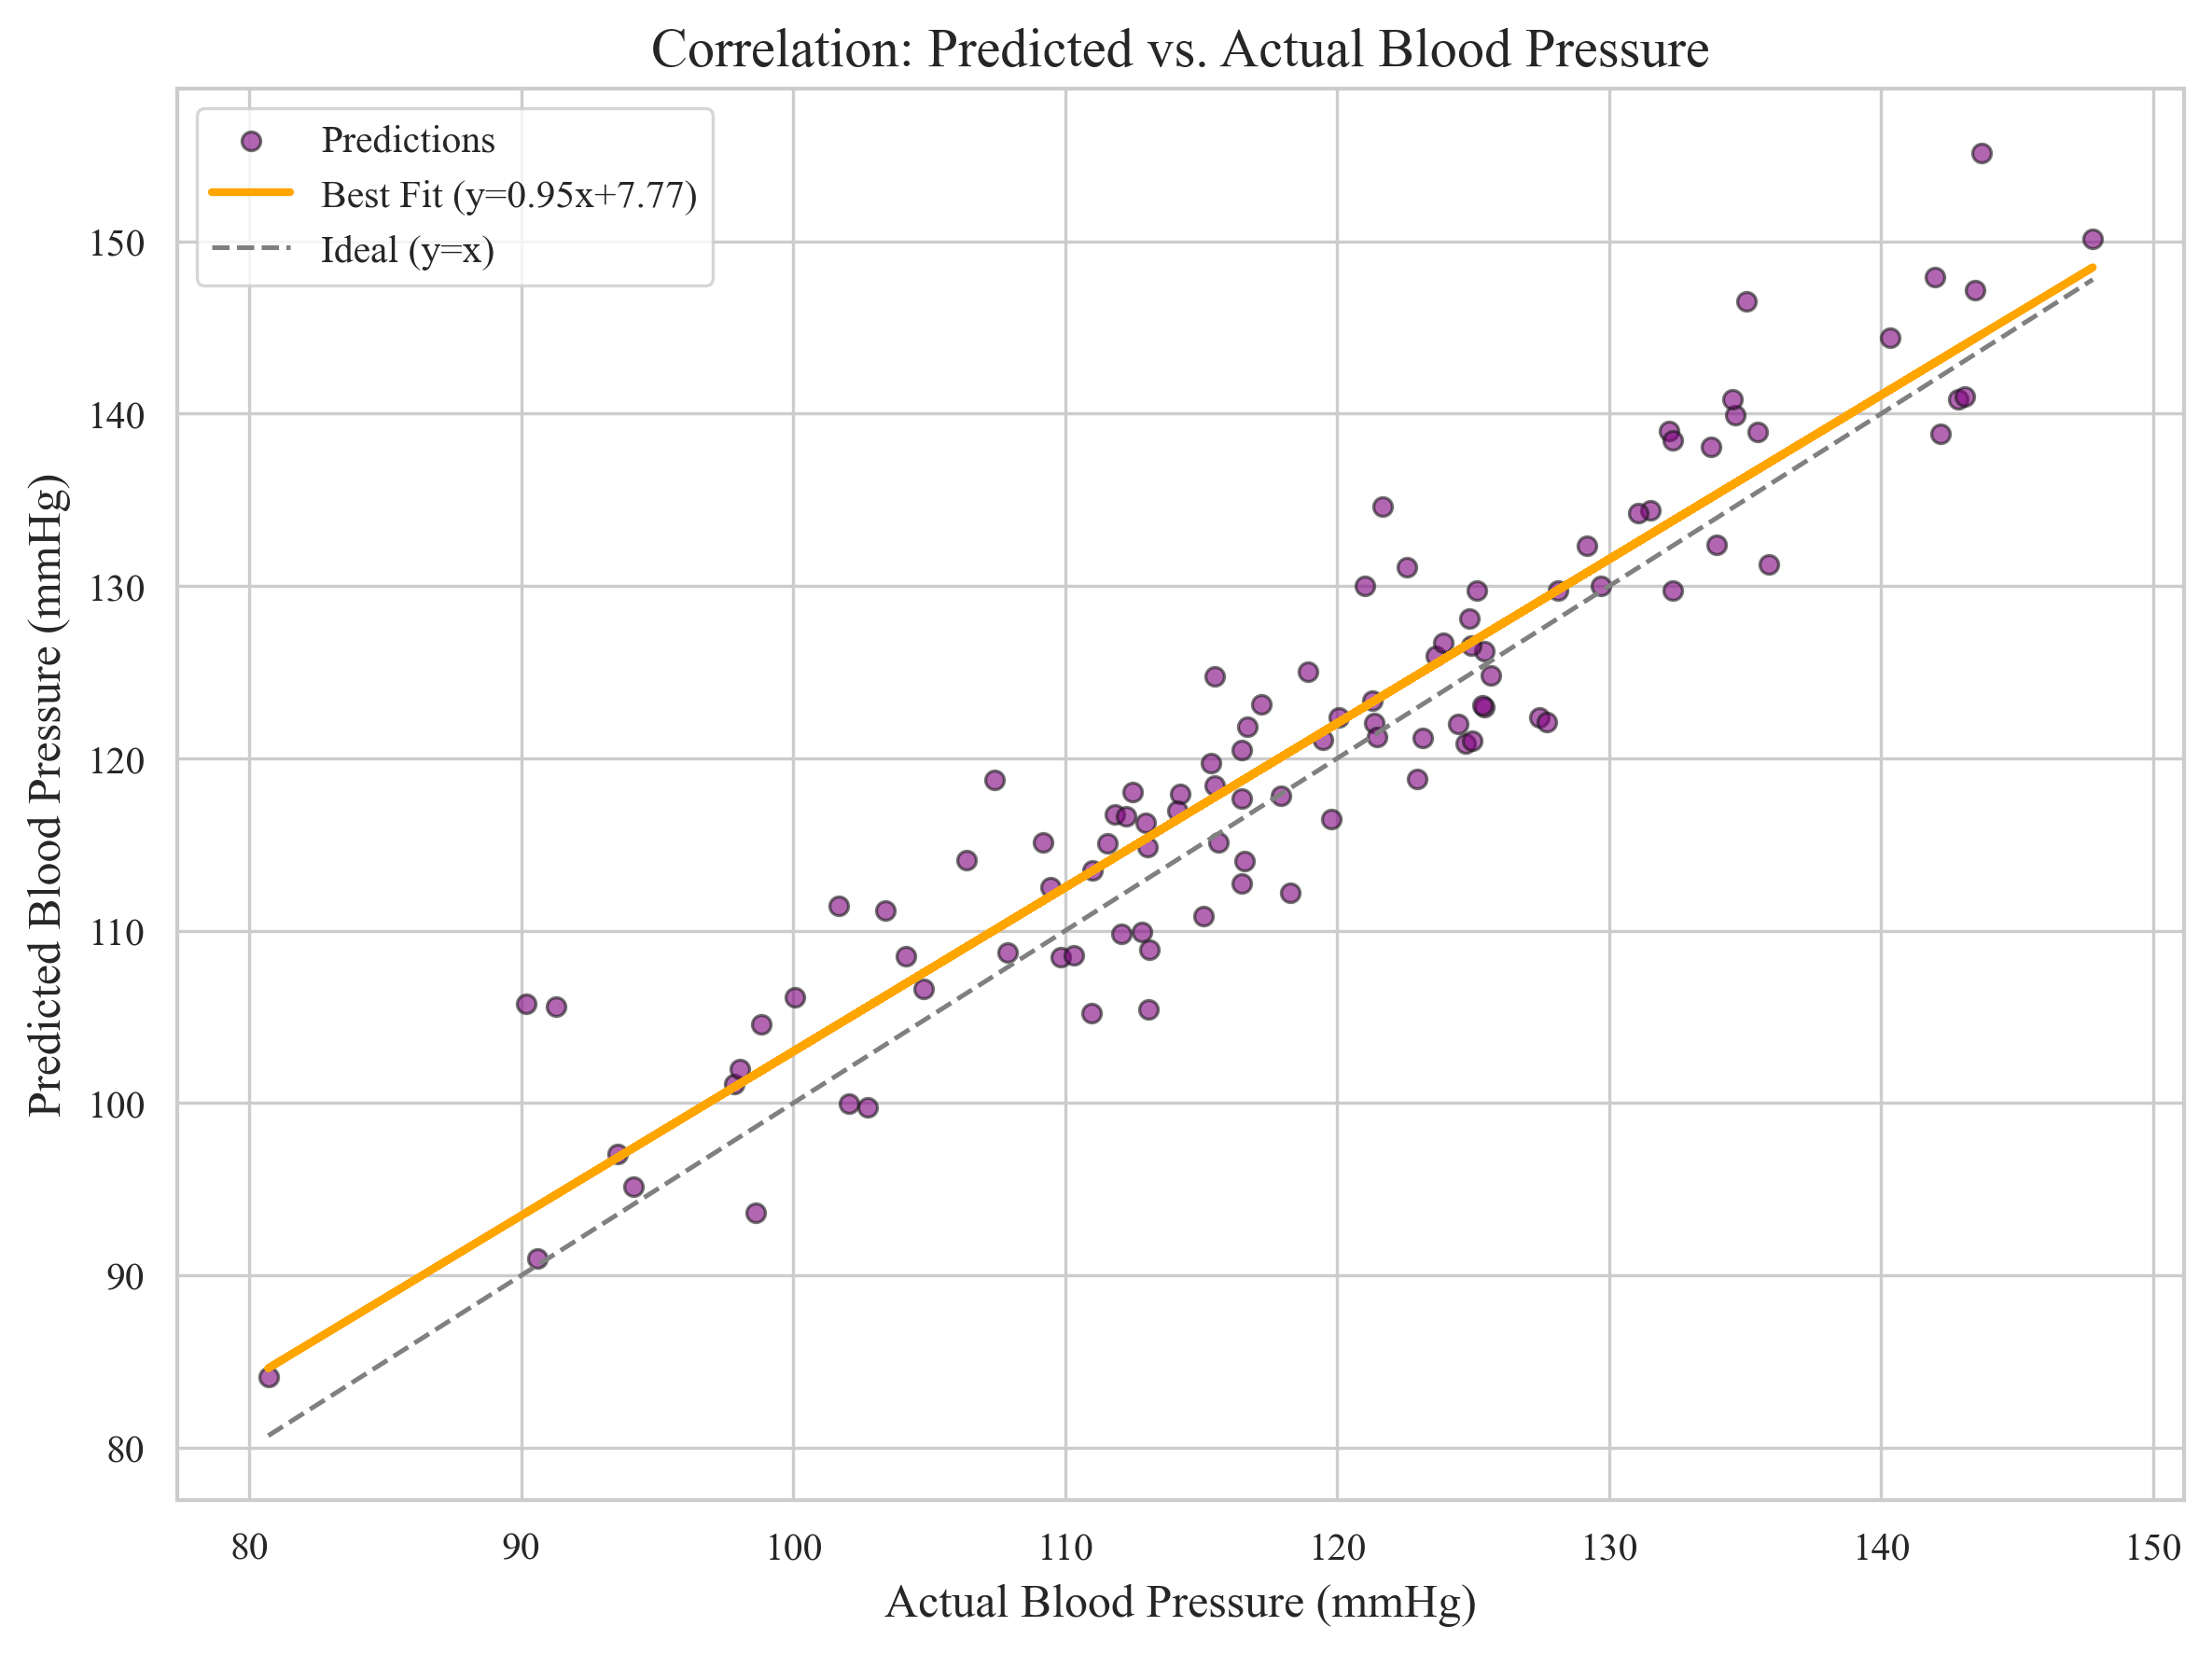
\includegraphics[width=\linewidth]{results/figures/fig4_correlation.png}
    \caption{Correlation Scatter Plot}
\end{subfigure}
\caption{Statistical agreement analysis. (a) The Bland-Altman limits of agreement demonstrate tight bounds for DBP. (b) The correlation scatter plot confirms the model escapes the regression-to-the-mean trap, accurately tracking hypertensive outliers.}
\label{fig:bland_altman}
\end{figure}

\subsection{Ablation Analysis}
Ablation studies confirm the necessity of our architectural choices. Removing the Savitzky-Golay filter and relying solely on Butterworth IIR filtering degraded DBP MAE by approximately 0.48 mmHg due to the distortion of the dicrotic notch. Furthermore, employing a monolithic joint regression head rather than the decoupled \textit{SepHead} design exacerbated regression-to-the-mean, artificially inflating the error on hypertensive outliers.

\section{Conclusion}

In this paper, we introduced LuminaBP, an end-to-end framework for non-contact, continuous blood pressure estimation from facial RGB video streams. By coupling strict exposure-locked optical acquisition, POS chrominance projection, and adaptive Savitzky-Golay morphological preservation, we successfully extracted high-fidelity 1D BVP signals. Our decoupled deep sequential network, MODEL-06-SepHead, independently modeled SBP and DBP pathways, mitigating gradient interference and template collapse.

Experimental validation on a large-scale, subject-independent cohort demonstrated an unprecedented Diastolic BP MAE of 5.91 mmHg, achieving compliance with the stringent ISO/AAMI SP10 clinical standard. Furthermore, successful deployment via 8-bit quantized TFLite on mobile Android hardware verifies the system's readiness for Edge AI inference.

While the current system achieves clinical accuracy for normotensive and moderately hypertensive subjects, future work must address extreme hypotensive and severe hypertensive outliers, potentially through Bayesian uncertainty quantification and personalized few-shot calibration. LuminaBP establishes a highly robust, scalable foundation for the next generation of ubiquitous, non-invasive cardiovascular digital biomarkers.


\bibliographystyle{IEEEtran}
\bibliography{references}

\end{document}
